\documentclass{article}
\usepackage[utf8]{inputenc}
\usepackage[top=1in, bottom=1in, left=1in, right=1in]{geometry}
\usepackage[style=authoryear,sorting=nyt]{biblatex}
\usepackage{graphicx}
\usepackage{multicol}
\usepackage{amsmath}

\title{Tweet classification and generation using dense, recurrent, and convolutional deep models}
\author{Shishir Tandale}
\date{May 2017}
\addbibresource{bib/technical.bib}

\begin{document}
\maketitle

\section{Related Work}
	Twitter data has historically been difficult to perform classification and generation
	tasks on. Twitter's users do their best to fit their messages within 140 characters
	by abbreviating and misspelling words, using hashtags and emoticons, and by quoting,
	retweeting, and by replying to themselves and others to keep the conversation going.
	Traditional natural language processing approaches are not as successful on Twitter
	data because of this noisiness in the data, and most approaches aim to correct this
	noise before feeding it into a model.

	Some data pre-processing tasks utilized in research and industry include removing
	low and high frequency words, keyword stemming, spelling correction, named entity
	recognition, and synonym replacement. These data pre-processing tasks certainly
	increase the effectiveness of models that use them, but can also slow down data ingestion
	due to increased processing time and lead to models that learn more simplified language
	structures. With this in mind, there is an incentive to using a model that can
	handle the noise in Twitter data requiring only minimal pre-processing to effectively
	learn a classification task or how to generate a Tweet indistinguishable from the input
	dataset. This paper explores different methods of enhancing text representations
	for the purposes of performing classification or generation using both word-level
	and character-level models.

	\subsection{Dense Representations}
		One common improvement on text classification tasks is using embeddings to help the
		model learn richer representations of text data. GloVe embeddings, used in this paper,
		are trained by modeling word co-occurrence probabilities and learning high-dimensional
		embedding vectors whose dot products equal the log probability of the words' co-occurrence
		\parencite{Pennington2014}. Instead of assigning integer ids to each word
		in order of their frequency, word embeddings are used instead and allow for more
		information about each word to be encoded \parencite{Baldi2012}. This approach allows for even simpler models
		like a multilayer perceptron to effectively model the relationship between words
		and any output can just be looked up in the embedding table via an optimized
		nearest neighbor search.

		Combining these word embeddings into sentence, document, or tweet embeddings is
		another challenge. One approach is to simply average together all of the composite
		word vectors, which disregards the order of the words in the collection. Another approach
		is to use an autoencoder architecture composing of an encoder and decoder. The
		encoder produces a vector representation of a sentence which the decoder uses
		to reproduce the input sentence . In NLP, recurrent networks
		like LSTMs are most often used as the encoder and decoder. This is done to deal
		with long term dependencies in text data such as pronouns and named entities,
		as recurrent networks continually learn a distribution's temporal structure.

		Producing these dense representations of tweets is important for prediction
		and classification tasks, as a good representation should encode a lot of information
		about the input but should still be compact enough to be memory efficient.
		An improvement on autoencoders is to enforce a particular distribution on the latent
		vectors. Variational autoencoders achieve this by using Kullback-Leiber (KL)
		divergence to measure the difference between the probability distributions of the
		encoder's latent representation, and an easy to deal with distribution like
		the unit Gaussian (with $\mu=0$, $\sigma=1$). This extra step ensures the
		encoder is producing vectors that all fit into a consistent space so the decoder
		learns how to map vectors from the unit Gaussian distribution to a sequence of
		characters or words. However, in practice, text generation on Twitter is still a very
		difficult problem due to the inherent noisiness in tweets between users, locations,
		topics, and style, leading to an incentive to improve the quality of generated text.

	\subsection{Generative Adversarial Networks}
		In computer vision, convolutional networks are frequently used
		to spatially sample nearby data to each point. Recent computer vision papers even
		push towards using generative adversarial networks (GANs) \parencite{Goodfellow2014}.
		GANs are a combination of a generator and discriminator network; the generator creates
		output data, $x^*=g(z)$, based on a random noise input, $z$, while the discriminator
		compares the output of the generator with a real image from the dataset, $x$, aiming to
		classify the generator's outputs as fake and the target dataset as real while the generator
		aims to fool the discriminator. This architecture allows for better image generation
		due to the complex training objectives that try to ensure controlled cooperation
		between the generator and discriminator through what is essentially a two-player
		minimax game.

		Deep convolutional GAN (DCGAN) \parencite{Radford2015} uses a stack of strided
		convolutions to create images from an input of random noise and a stack of
		regular convolutions to determine which images are real and fake. DCGAN is highly
		effective at producing images that reasonably look like they came from the same
		input dataset, however it still exhibited issues like mode collapse which results
		in outputs that all resemble a single class of input. Mode collapse arises when
		$g(z)=x_m$ is the same for many $z$ across the random distribution $p(z)$, so
		ensuring the generator responds to it's noise input is key in preventing mode collapse.

		One key improvement of DCGAN was Wasserstein GAN (WGAN) \parencite{Arjovsky2017}
		which replaced the KL divergence used in GANs to measure differences between generated
		samples and training samples with the Wasserstein distance. The results are impressive --
		training times decreased, the model was less sensitive to network structure, and output
		images looked perceivably nicer and fit closer to the input dataset, without exhibiting mode collapse.
		Switching DCGAN architectures to WGAN seems like a simple decision to make, but there
		are many properties of the Wasserstein distance that apply to fields outside of
		computer vision.

		One unintended side effect of using the Wasserstein distance instead of KL divergence is that distances
		between two probability distributions are represented continuously. This allows
		for WGANs to more effectively generate text data because the calculated gradients
		from the generator's output is continuous even considering the discretized nature of text
		\parencite{GoodfellowReddit2016}. WGAN, unlike more traditional variations of GAN using
		KL divergence, can be effective at generating text that looks like the target distribution.

	\subsection{Adversarial Autoencoders}
		However, for classification purposes, GANs are not as useful because there is no
		structure imposed on the random input noise to the generator, besides the distribution
		it is sampled from. Randomly sampling the generator simply yields data that looks like
		the training set. However, outputs that all	fall under a specific class can be created
		by depth concatenating the class label to the generator's input noise and as part of
		the discriminator's convolutional feature maps. Doing so essentially determines
		part of the generator's prior probability distribution ahead of time, so an alternative
		approach might be to use variational autoencoders (VAEs) to enforce a particular
		probability distribution to begin with.

		By training a VAE to encode a sentence into a latent vector, we can use the decoder
		to decode arbitrary vectors sampled from the same latent space enforced by the VAE.
		We can achieve better performance by adding a discriminator network that determines
		whether or not a latent vector $z$ comes from the encoder network's distribution $q(z|x)$ or is drawn
		from the target probability distribution $p(z)$ \parencite{Makhzani2015}.
		The same concept of merging generative adversarial networks with variational autoencoders
		was also explored by \cite{Mescheder2017} which used a slightly different model
		structure and dives deeper into the theoretical justification behind their
		approach.

		These combined models are called adversarial autoencoders (AAEs) and result in
		a decoder that can effectively sample from all across $p(z)$ since the adversarial
		component was designed to ensure $q(z|x)$ spans as much of $p(z)$ as possible
		such that an arbitrary $z \sim p(z)$ results in a meaningful sample when passed through
		the decoder. This is shown best by the diagrams in both \cite{Makhzani2015} and
		\cite{Mescheder2017}, which compares the output of their AAEs compared with
		traditional variational autoencoders. AAE latent vectors are much more consistently
		organized across the various classes of input data, and this more structured
		space is easier to produce good text samples from through the decoder.

\section{Models}
	\begin{figure}
		\centering
			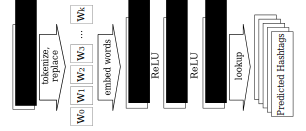
\includegraphics[width=0.8\textwidth]{figures/baseline_model}
		\caption{Structure of MLP model with 50 hidden layer nodes and
			GloVe size of 25.}
	\end{figure}

	\subsection{MLP Classifier}
		In order to predict likely hashtags for a given tweet $t \in Tweets$, we first
		tokenize our text and replace tokens like Twitter user references, URLs, and
		hashtags with GloVe tags like \verb|<user>|, \verb|<url>|, and \verb|<hashtag>|.
		Next, we embed all of our tokens using a GloVe Twitter dataset, replacing
		unknown tokens with zero vectors, and average together all of the word embeddings
		to form a sentence embedding. Alternatives like vector sums or concatenation
		may be better ways to calculate tweet or sentence embeddings \parencite{Garten2015}, but since we are finding
		a transformation between average word space and hashtag space, a simple averaging
		operation gives us good results anyway. For a given hashtag $h \in Hashtags$, and associated tweets
		$T_h$, the hashtag embedding $E(h)$ is defined as the average of all the associated
		tweet embeddings:

		$$E(h) = \frac{1}{|T_h|}\sum_{t\in T_h} E(t)$$

		Once all of the embeddings are calculated, tweets are paired up with their hashtags
		such that if $t_1$ contained $h_1$, $h_2$, and $h_3$, then the input pairs to our
		classifier $C$ are $(t_1, h_1), (t_1, h_2),$ and $(t_1, h_3)$. Let the total collection of
		all pairs be $p$, such that $\left(E(t_i), E(h_j)\right)\in p \Leftrightarrow t_i\in T_{h_j}$,
		which makes $p$ a collection of all valid tweet-hashtag embedding pairs. Batches of $p$ are used
		as the input for the network. Notice that for separate pairs $p_a, p_b \in p$, $p_a$ and $p_b$
		can share the same exact tweet embedding with different hashtag embeddings. When processed
		this way, we can think of this classifier as incrementally learning how to transform each
		tweet embedding into each one of its hashtag embeddings. This works because we have fewer
		hashtags than tweets, so the model has an easier time learning to map to this smaller space.
		Adam \parencite{Kingma2014} was used to train this network. The loss was calculated by
		calculating the L2 loss, or the sum of squared differences:

		 $$\text{L2\_loss} = \sum_{(E_t, E_h)\in \text{batch}} \left(C(E_t) - E_h\right)^2$$

		As shown in Figure 1 above,
		The classifier $C$'s structure consists of two fully-connected hidden layers with
		$2\cdot$(\verb|glove_embedding_dim|) neurons each, each feeding into a ReLU. The output
		layer has \verb|glove_embedding_dim| neurons and does not use any normalizing
		functions like softmax because instead of a probability, we want a vector in hashtag
		embedding space. These predictions are parsed by performing a nearest neighbors search
		on our list of embedded hashtags by using a ball tree data structure for efficiency.

	\subsection{LSTM Generator}
	\subsection{Wasserstein AAE Generator}

\section{Dataset}
	The dataset used was datahub.io's Twitter 2012 Presidential Election dataset. This
	dataset comes in the form of compressed json files each with between a million and
	a billion status JSON records. In addition to an existing data set, this project
	also can use Tweepy as a client to download tweets from a particular user or search term,
	and to stream tweets in real-time with arbitrary search terms. This allows a
	very recent dataset to be amassed rather quickly, and in a format already suitable
	for the data processing pipeline.

	Pre-trained 25-dimensional word vectors were obtained from GloVe's Twitter dataset,
	which was taken over two billion tweets and a vocabulary of size 1.2 million.

	\subsection{Pipeline Implementation}
		In order to efficiently parse the data in a form usable by all of the networks discussed
		in this paper, an object-oriented class structure that modeled the relationship between tweets and
		hashtags was created. A TwitterProperty super class manages all of the data structure
		membership logic while the implementing Tweet and Hashtag classes specify
		their own variables used to calculate their hashes. This is important because
		these same hashes are used to compute set membership to prevent duplicate hashtags.
		This is done by overriding the hash method in the TwitterProperty super class to
		look at the string representation of the object. The Tweet and Hashtag classes
		inherit this hash method, so all they need to do is override their to-string method
		to use the raw text provided on object initialization. This creates hash collisions
		even though the objects being stored are unique, and when this happens, an object
		reference that caused the hash collision is replaced with the reference already in the dictionary.

		This results in consistent references to unique tweets and hashtags to be saved
		while all duplicate objects are thrown away. This also allows any other class
		to access the static data structures part of the Tweet and Hashtag classes, retrieving
		a reference to the global list of Tweets and Hashtags, complete with references
		to their embeddings and other connected Tweets and Hashtags. This results in
		loosely coupled code with different objects for JSON processing, tweet tokenization,
		and tweet/hashtag storage that is also very efficient in Python 3.6 thanks to
		an improved dictionary implementation. Modifying this pipeline for earlier
		versions of Python is problematic due to this heavy reliance on data structures
		which are more efficiently implemented in 3.6 and newer.

	\subsection{Pre-model Processing}
		For tweets we want to embed, regex is used to strip hashtags, user references,
		and URLs from tweets, replacing them with the appropriate GloVe tags. This is done
		because those elements are not likely to be in our GloVe embedding lookup table
		but it is important our model understands the significance of the missing tokens.
		This is done automatically by the Tweet class upon creating a Tweet object.

		For the AAE and LSTM models, tweets are broken up by character and encoded by character
		frequency before being padded with empty tokens and shaped for the assigned batch
		size. Theoretically, using our already generated embeddings should result in
		better results, but character-level models tend to have higher flexibility in
		generating outputs, which is valuable for this paper's purposes.

\section{Results}
	\subsection{MLP Classification}
	\subsection{LSTM Generation}
	\subsection{AAE Generation}

\section{Analysis}
	\subsection{MLP Classification}
	\subsection{LSTM Generation}
	\subsection{AAE Generation}

\printbibliography
\end{document}
